\documentclass[11pt,a4paper]{article}
\usepackage[utf8]{inputenc}
\usepackage{amsmath,amssymb,amsthm,amsfonts,enumerate,enumitem}
\usepackage{graphicx}
\usepackage[margin=1in]{geometry}
\usepackage{subcaption}
\usepackage[numbib]{tocbibind} % To number the References section
\usepackage{tikz,pgfplots}
\usepackage{tikzpagenodes}
\usepackage{algorithm2e}
\usepackage{algorithmic}
\usepackage{animate}


\usepackage{soul}

%%%%%%%%%%%  Tikz libraries  %%%%%%%%%%%%%%%% 

\usetikzlibrary{positioning,automata}
\usetikzlibrary{matrix}
\usetikzlibrary{arrows,shapes}
\usetikzlibrary{trees}
\usetikzlibrary{backgrounds}
\usetikzlibrary{shapes.geometric}
\usetikzlibrary{calc,shapes.callouts,shapes.arrows}
\usetikzlibrary{graphs}
\usetikzlibrary{positioning, arrows}
\usetikzlibrary{fit}


%%%%%%%%%%%  Environments  %%%%%%%%%%%%%%%% 

\newtheorem{theorem}{Theorem}[section]
\newtheorem{lemma}[theorem]{Lemma}
\newtheorem{proposition}[theorem]{Proposition}
\newtheorem{conjecture}[theorem]{Conjecture} 
\newtheorem{cor}[theorem]{Corollary}
\newtheorem{example}[theorem]{Example}
\newtheorem{rem}[theorem]{Remark}
\newtheorem{definition}[theorem]{Definition}
\newtheorem{conj}{Conjecture}[section]
% \newtheorem{procedure}{Procedure}[section]
\newtheorem{question}{Question}[section]
\newtheorem{claim}{Claim}[section]
\newtheorem{quest}{Question for US}[section]
\theoremstyle{definition}


\title{MATH 4920 -- Undergraduate Research Projects\\
{\small{Manitoba eXperimental Mathematics Laboratory}}\\
\vspace{3mm}
\textbf{Exploring perfect binary trees with relation to the HK-property}}

\author{Atishaya Maharjan\\
Supervisor: Dr. Mahsa N. Shirazi\\
}

\date{Winter 2024}

\begin{document}

\maketitle

\section{Introduction}

For a given graph $G = (V,E)$, $V(G)$ and $E(G)$ denotes the vertex sets and edge sets of the graph $G$. For an arbitrary vertex, $v \in V(G)$, all vertices adjacent to $v$ by an edge are called the neighbours of $v$ and is denoted by $N_G(v)$. The degree of a vertex $v \in V(G)$ is the cardinality of the set of neighbours of $v$, and is denoted by $deg_G(v)$.

For $n \in \mathbb{Z^+}$ such that  $0 \leq n \leq |V(G)|$, a path of length $n$ in $G$ is a sequence of distinct vertices $v_1, v_2, \ldots, v_n$ such that $v_i$ is adjacent to $v_{i+1}$ for $1 \leq i \leq n-1$. A cycle is an extension of a path such that the last vertex is connected to the first vertex, i.e for a path of length $n$, $v_nv_i \in E(G)$. As such, the length of the cycle is $n + 1$.

A connected graph is a graph if for all $u,v \in V(G)$, there exists a $uv$-path. An coclique is a set of vertices such that no two vertices in the set are adjacent to each other. It is denoted by $I$. We denote a family of indpendent sets of a graph $G$ as $I_G$. A family of coclique of a graph $G$ of cardinality $n$ is denoted by $\mathcal{I}^n_G$. For $v \in V(G)$, the family of indpendent sets, $\mathcal{I}^n_G(v) := \{A \in \mathcal{I}^n_G : v \in A\}$ is called a star of $\mathcal{I}^n_G$ and $v$ is called its center.

A tree is a connected graph with no cycles, it is denoted by $T$. For a vertex $v \in V(T)$, if $deg_T(v) = 1$, it is called a leaf. A vertex that is not a leaf is called an interior vertex. The depth of a vertex is defined as length of the path from the root vertex to it. We study a more particular class of trees called binary trees, denoted by $T_B$, where each interior vertex $v$ has exactly $2$ children and all leaves have the same depth. Further, a perfect binary tree is a binary tree in which every vertex $v \in V(T)$ has either $0$ or $2$ children. A perfect binary tree is denoted by $T_{PB}$, however in this report we will simply drop the subscript and denote it as $T$ for clarity. A level $n$ of a perfect binary tree is a set of vertices such that all vertices in the set have a depth of $n$.

The star centers of a graph are interesting because they relate to the EKR theorem.

\section{Background and Project Goals}

The Erd\H{o}s-Ko-Rado (EKR) theorem limits the number of sets in a family of sets that can be pairwise intersecting. The theorem states that for a family of $k$-sets, the maximum number of sets that can be pairwise intersecting is $\binom{n-1}{k-1}$. This theorem has wide applications in combinatorics, graph theory, probability, and other areas of statistics and mathematics.

Studying the EKR theorem, $\cite{MR2763040}$ Hulbert and Kamat conjectured the following:

\begin{conjecture}[k-EKR Conjecture]
	Let $G$ be a graph, and let $\mu(G)$ be the size of its smallest maximal coclique. Then $G$ is $k$-EKR for every $1 \leq k \leq \frac{\mu(G)}{2}$.
\end{conjecture}

However, even this conjecture is hard to understand and prove, so they narrowed the class of graphs to be trees and gave the following conjecture:

\begin{conjecture}[HK-Property]
	For any $k \geq 1$ and any tree $T$, there exists a leaf $l$ of $T$ such that $|\mathcal{I}^k_T(v)| \leq |\mathcal{I}^k_T(l)|$ for each $v \in V(T)$.
\end{conjecture}

The HK-property holds true for $k \leq 4$, but was proven false independetly by ~\cite{MR3271819, MR3612439, MR2523796}. The counterexample that that they arrived at is a type of graph that is defined as a class of trees called "lobsters" ~\cite{MR4245360}. This is interesting for us as the counterexample graph resembles a binary tree.

\begin{figure}
	\centering
	\begin{tikzpicture}[scale=0.7,level distance=2cm,
			level 1/.style={sibling distance=8cm},
			level 2/.style={sibling distance=4cm},
			level 3/.style={sibling distance=2cm},
			every node/.style={circle, draw, fill=white, minimum size=1.75em},]
		\node (v11) {$v_0$}
		child {node (v21) {$v_1$}
				child {node  {}
						child {node {}}
					}
				child {node (v32) {}
						child {node {}}
					}
			}
		child {node (v22) {$v_2$}
				child {node (v33) {}
						child {node {}}
					}
				child {node (v34) {}
						child {node {}}
					}
			};
	\end{tikzpicture}
	\caption{The largest k-star for $k \geq 5$ is centered at $v_0$}
\end{figure}

They figured out that the lobsters, while not completely obeying the HK-property, almost obey the HK-property by either having the largest stars centered around the leaves or at the root of the tree.

Henceforth, we shall give a name to the property that the largest stars are centered around the leaves or the root of the tree as:

\begin{definition}[Partial HK-Property]
	If a tree $T$ has the property that for any $k \geq 1$, there exists a leaf $l$ of $T$ such that $|\mathcal{I}^k_T(v)| \leq |\mathcal{I}^k_T(l)|$ for each $v \in V(T)\setminus\{r\}$, where $r$ is the root, then we say that $T$ satisfies the Partial HK-Property.
\end{definition}

Since the binary trees are very similar in structure with the lobsters, the overall goal of this research was to figure out if the HK-property or the Partial HK-Property holds for perfect binary trees.

In the paper by Estrugo and Passtine~\cite{MR4245360}, they gave a couple of classes of graphs that have the HK-property. The classes of graphs that they gave were the caterpillars and the stars.

\begin{figure}[htb!]
	\begin{minipage}{0.5\textwidth}
		\centering
		\begin{tikzpicture}[every node/.style={circle, draw, fill=white, minimum size=1.75em}]
			% Draw the path (spine)
			\node (v1) at (0,0) {$v_1$};
			\node (v2) at (2,0) {$v_2$};
			\node (v3) at (4,0) {$v_3$};
			\node (v4) at (6,0) {$v_4$};
			\draw (v1) -- (v2) -- (v3) -- (v4);

			% Draw the leaves
			\node (v7) at (4,2) {$v_7$};
			\node (v8) at (6,2) {$v_8$};
			\node (v9) at (6,-2) {$v_9$};  % New vertex attached to v4
			\draw (v3) -- (v7);
			\draw (v4) -- (v8);
			\draw (v4) -- (v9);  % Edge to the new vertex
		\end{tikzpicture}
		\caption{A caterpillar}
	\end{minipage}
	\begin{minipage}{0.5\textwidth}
		\centering
		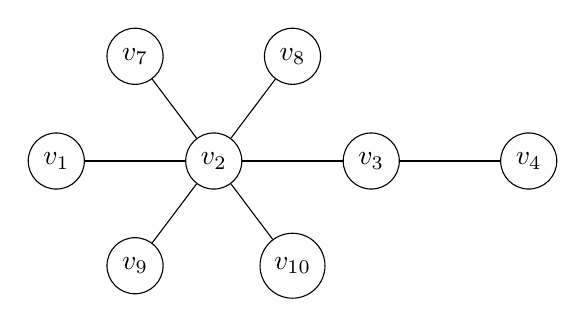
\begin{tikzpicture}[every node/.style={circle, draw, fill=white, minimum size=1.75em}]
			% Draw the path (spine)
			\node (v1) at (0,0) {$v_1$};
			\node (v2) at (2,0) {$v_2$};
			\node (v3) at (4,0) {$v_3$};
			\node (v4) at (6,0) {$v_4$};
			\draw (v1) -- (v2) -- (v3) -- (v4);

			% Draw the leaves
			\node (v7) at (1,1.33) {$v_7$};
			\node (v8) at (3,1.33) {$v_8$};
			\node (v9) at (1,-1.33) {$v_9$};
			\node (v10) at (3,-1.33) {$v_{10}$};
			\draw (v2) -- (v7);
			\draw (v2) -- (v8);
			\draw (v2) -- (v9);
			\draw (v2) -- (v10);
		\end{tikzpicture}
		\caption{A Spider}
	\end{minipage}
\end{figure}

The caterpillars are trees that have a path as the spine and the leaves are attached to the spine. The spiders are trees that only have 1 vertex with degree greater than 2.

They also proved that the Lobsters satisfy the Partial HK-Property.

\section{Ideas}

\subsection{Idea: Flip functions and escape paths}

Estrugo and Passtine~\cite{MR4245360} proved all the classes of graphs that satisfy the HK-property by using a \textbf{flip function} alongside the idea of an \textbf{escape path}.

\begin{definition}[Escape path]
	Let $G$ be a graph and $P = v_1,v_2,\ldots,v_n$ be a path of length $n$ such that $P \subset G$. We say that $P$ is an escape path from $v_1$ to $v_n$ in $G$ if $deg(v_n) = 1$ and $deg(v_i) = 2$ for all $i \in \{2,3,\ldots,n-1\}$. If this is the case, then we say that $P$ is an escape path from $v_1$ to $v_n$ in $G$.
\end{definition}

\begin{definition}[Flip function]
	Let $G$ be a graph and $P = v_1,v_2,\ldots,v_n$ be an escape path from $v_1$ to $v_n$ in $G$. Then the flip of $P$ in $G$, \text{flip}$_P$ : $V(G) \rightarrow V(G)$ is the function defined as follows:

	\begin{align*}
		\text{flip}_P(v) = \begin{cases}
			                   v             & \text{if } v \not\in V(P)   \\
			                   v_{n + 1 - i} & \text{if } v = v_i \in V(P) \\
		                   \end{cases}
	\end{align*}
\end{definition}

Using the two definitions, they showed that the flip$_P$ induces a one to one mapping from $\mathcal{I}^k_G(v_1)$ to $\mathcal{I}^k_G(v_n)$. By showing that the flip function is an injection, they then used the Cantor-Schröder-Bernstein theorem to show that the $|\mathcal{I}^k_G(v_1)| \leq |\mathcal{I}^k_G(v_n)|$

By that, they showed that the classes of graphs that they gave satisfy the HK-property and that the lobster graphs satisfy the Partial HK-Property.

So, our idea was to use the flip function and the escape path to show that the perfect binary trees satisfy the HK-property or the Partial HK-Property. Our initial idea was to use a ``diagonal'' flip function that would flip the vertices along the diagonal of the perfect binary tree. To do this, we would have to address 4 important points:

\begin{enumerate}
	\item Enumerate the vertices of the perfect binary tree in a way that the new flip function would be able to map them around.
	\item Define an escape path that would be able to escape from the root to the leaf of the perfect binary tree.
	\item Define a flip function that would flip the vertices along the diagonal of the perfect binary tree.
\end{enumerate}

\subsubsection*{Enumerate the vertices of the perfect binary tree in a way that the new flip function would be able to map them around.}

\begin{definition}[Depth Vertex]
	Let $\mathcal{V}_k \in V(T)$ be the set of vertices of depth $k$. We call $\mathcal{V}_k$ as the depth vertex set of depth $k$. Index all vertices in $\mathcal{V}_k$ from left to right as $v_{k, i}$, where $k$ is the depth of the vertex and $i$ is the index of the vertex in $\mathcal{V}_k$ such that $1 \leq i \leq 2^{k - 1}$.
\end{definition}

\begin{figure}
	\centering

	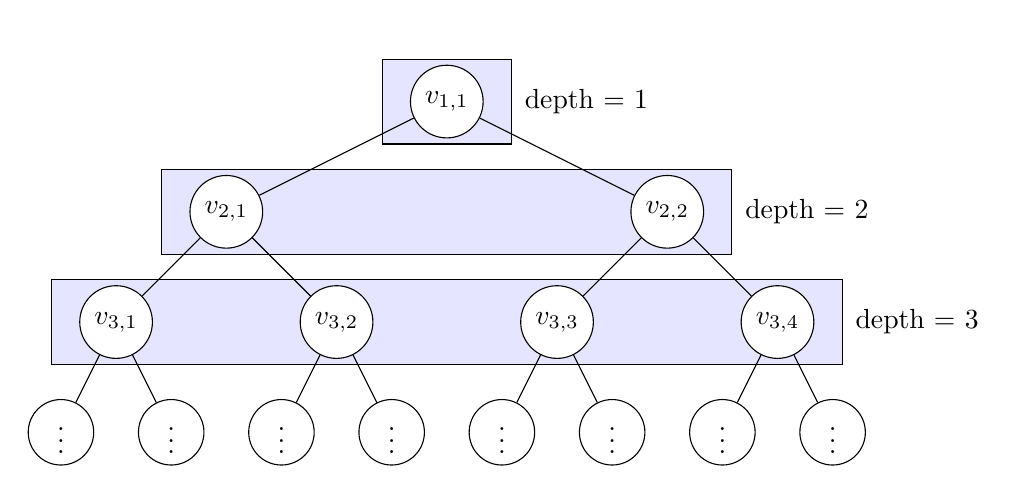
\begin{tikzpicture}[scale=0.7,level distance=2cm,
			level 1/.style={sibling distance=8cm},
			level 2/.style={sibling distance=4cm},
			level 3/.style={sibling distance=2cm},
			every node/.style={circle, draw, fill=white}]
		\node (v11) {$v_{1,1}$}
		child {node (v21) {$v_{2,1}$}
				child {node (v31) {$v_{3,1}$}
						child {node {$\vdots$}}
						child {node {$\vdots$}}
					}
				child {node (v32) {$v_{3,2}$}
						child {node {$\vdots$}}
						child {node {$\vdots$}}
					}
			}
		child {node (v22) {$v_{2,2}$}
				child {node (v33) {$v_{3,3}$}
						child {node {$\vdots$}}
						child {node {$\vdots$}}
					}
				child {node (v34) {$v_{3,4}$}
						child {node {$\vdots$}}
						child {node {$\vdots$}}
					}
			};

		\begin{scope}[on background layer]
			\node[draw,rectangle,fit=(v11),inner xsep=10pt, inner ysep=2pt, fill=blue!10, label=right:{depth = 1}] {};
			\node[draw,rectangle,fit=(v21) (v22),inner xsep=10pt, inner ysep=2pt, fill=blue!10, label=right:{depth = 2}] {};
			\node[draw,rectangle,fit=(v31) (v32) (v33) (v34),inner xsep=10pt, inner ysep=2pt, fill=blue!10, label=right:{depth = 3}] {};
		\end{scope}
	\end{tikzpicture}
\end{figure}

\subsubsection*{Define a flip function that would flip the vertices along the diagonal of the perfect binary tree.}

To save ourselves the trouble of defining a flip function for every path,, we decided to define an auxilary function that would flip the vertices along the vertex set so that our choice of vertices in the diagonal flip function would be arbitrary.

\begin{definition}[Flip Function on Depth Vertex Set]
	Let $T$ be a perfect binary tree and $\mathcal{V}_k$ be the depth vertex set of depth $k$. Then, the flip of $\mathcal{V}_k$ in $T$, denoted by $flip_\mathcal{K}: \mathcal{V}_k(G) \rightarrow \mathcal{V}_k(G)$, is the function defined as follows:

	\begin{equation*}
		flip_\mathcal{K}(v_{(k, i)}) = \begin{cases}
			v_{(k, 2^{k-1} + 1 - i)}  & \text{if } N_T(v_{(k, 2^{k - 1} + 1 - i)}) \not\subseteq \mathcal{I}_T(v_{(k, 2^{k - 1} + 1 - i)}) \\
			v_{(k, 2^{k-1} + 1 - i)}, & \text{if } N_T(v_{(k, 2^{k - 1} + 1 - i)}) \subseteq \mathcal{I}_T(v_{(k, 2^{k - 1} + 1 - i)})     \\
			flip_N(v_{(k, i)}),       & \text{if } N_T(v_{(k, 2^{k - 1} + 1 - i)}) \subseteq \mathcal{I}_T(v_{(k, 2^{k - 1} + 1 - i)})
		\end{cases}
	\end{equation*}

	\text{where, $flip_N$ is defined as:}
	\begin{equation*}
		flip_N(v_{(k, i)}) =  flip_\mathcal{K}(u), \text{ for all } u \in N_T(v_{(k, i)})
	\end{equation*}
\end{definition}

We then have the following lemma:

\begin{lemma}[$flip_\mathcal{K}$ is a bijective involution]\label{lemma_flip_bijective_involution}
	Let $T$ be a perfect binary tree and $\mathcal{V}_k$ be the depth vertex set of depth $k$. Then, the flip function $flip_\mathcal{K}$ is an involution.
\end{lemma}
\begin{proof}
	Let $\mathcal{V}_k$ be the depth vertex set of depth $k$. Since the function is defined recursively, we can evaulate the flipping step and then show that the flip function on the neighbours of a vertex also results in an involution.

	We first evaluate the flipping step for when the neighbours of the vertex are not in the coclique. Then, applying the flip function twice, we have:

	\begin{align*}
		flip_\mathcal{K}(flip_\mathcal{K}(v_{k, i})) & = flip_\mathcal{K}(v_{(k, 2^{k-1} + 1 - i)}) \\
		                                             & = v_{(k, 2^{k-1} + 1 - (2^{k-1} + 1 - i))}   \\
		                                             & = v_{(k, i)}
	\end{align*}
	Hence, $flip_\mathcal{K}$ is an involution when the neighbours of the vertex are not in the coclique.

	We now have to show that the flip function on a vertex when the neighbours of the vertex are in the same coclique is also an involution.

	Consider a vertex, $v_{(k, i)}$, such that $N_T(v_{(k, 2^{k-1} + 1 - i)}) \subseteq \mathcal{I}_T(v_{(k, 2^{k-1} + 1 - i)})$. Then, when we apply the $flip_\mathcal{K}$ function twice, we obtain that:

\end{proof}

We then proceed to show that the flip function on a depth vertex set maps cocliques into cocliques.

\begin{lemma}\label{lemma_flip_independent_sets}
	Let $T$ be a perfect binary tree and $\mathcal{V}_k$ be the depth vertex set of depth $k$. Let $\mathcal{I}^m_{\mathcal{V}_k}$ be the family of cocliques of cardinality $m$. Then, the flip function $flip_\mathcal{K}$ maps cocliques into cocliques and induces a bijection from $\mathcal{I}^m_{\mathcal{V}_k}$ onto itself.

	In addition, $flip_\mathcal{K}(\mathcal{I}_{\mathcal{V}_k}(v_{k, 1})) = \mathcal{I}_{\mathcal{V}_k}(v_{k, 2^{k-1}})$.
\end{lemma}

\begin{proof}
	Let $\mathcal{I}$ be an coclique and assume two unique vertices $v_{k, i}, v_{k, j} \in flip_\mathcal{K}(\mathcal{I})$, i.e $i \neq j$. Since both $v_{k, i}$ and $v_{k, j}$ belong to the depth vertex set, and since this is a perfect binary tree, we see that $v_{k, i}$ and $v_{k, j}$ are not adjacent to each other. Hence, $flip_\mathcal{K}(\mathcal{I})$ is an coclique. Thus, $flip_\mathcal{K}$ maps cocliques into cocliques.

	Now, let $\mathcal{I}^m_{\mathcal{V}_k}$ be the family of cocliques of cardinality $m$ of the depth vertex set $\mathcal{V}_k$. Then, $flip_\mathcal{K}$ is a bijection from $\mathcal{I}^m_{\mathcal{V}_k}$ onto itself.

	Finally, we have $flip_\mathcal{K}(\mathcal{I}_{\mathcal{V}_k}(v_{k, 1})) = \mathcal{I}_{\mathcal{V}_k}(v_{k, 2^{k-1} + 1 - 1}) = \mathcal{I}_{\mathcal{V}_k}(v_{k, 2^{k-1}})$, as required.

	Hence, $flip_\mathcal{K}$ maps cocliques into cocliques and induces a bijection from $\mathcal{I}^m_{\mathcal{V}_k}$ onto itself.
\end{proof}


Now, our objective is to procure a similar result to ~\cite{MR4245360} to show that our flip function induces a one to one mapping from any family of coclique $\mathcal{I}_{T}(v)$ for any vertex $v \in V(T)$ into any family of coclique $\mathcal{I}_{T}(l)$ for a leaf $l \in V(T)$. We also need to define a diagonal flip function that will flip the vertices along the diagonal of the perfect binary tree. To do that, we will need to define an escape path that would be able to escape from the root to the leaf of the perfect binary tree.

\subsubsection*{Define an escape path that would be able to escape from the root to the leaf of the perfect binary tree.}

However, in our objective to properly define a diagonal flip function, we encountered a problem. The perfect binary trees does not have an escape path. The escape path is defined such that the middle vertices are all part of a pure path. This is not achievable in the perfect binary tree as all the interior vertices have 2 children, i.e. degree 3. Hence, we were unable to define an escape path that would be able to escape from the root to the leaf of the perfect binary tree.

\subsection{Algorithmic Approach}

To validate our conjecture, we present a simple algorithm to generate all cocliques of a perfect binary tree of cardinality $k$. We then compare the number of cocliques containing a vertex $v$ and a leaf $l$ to see if the HK-property holds for perfect binary trees.

To begin with, we present the following algorithm to generate a perfect binary tree of depth $n$:

\RestyleAlgo{ruled}

\SetKwComment{Comment}{/* }{ */}

\begin{algorithm}[hbt!]
	\caption{Perfect Binary Tree Generator}\label{alg:tree-generator}
	\KwData{$n \geq 0$, where $n$ is the depth of the perfect binary tree}
	\KwResult{A perfect binary tree graph and its leaves}

	\SetKwFunction{FMain}{perfect\_binary\_tree\_generator}
	\SetKwFunction{FSub}{get\_leaves}

	\SetKwProg{Fn}{Function}{:}{}
	\Fn{\FMain{$n$}}{
		\eIf{$n = 0$}{
			\Return{Graph()}
		}{
			$g \gets Graph()$\;
			$g$.add\_vertices([$2^n$])\;
			\For{$i$ in range($2^n - 1$)}{
				$g$.add\_edge($i$, $2*i + 1$)\;
				$g$.add\_edge($i$, $2*i + 2$)\;
			}
			\Return{$g$}
		}
	}
\end{algorithm}

\newpage

The algorithm will generate a perfect binary tree of this form:
\begin{figure}[hbt!]
	\centering

	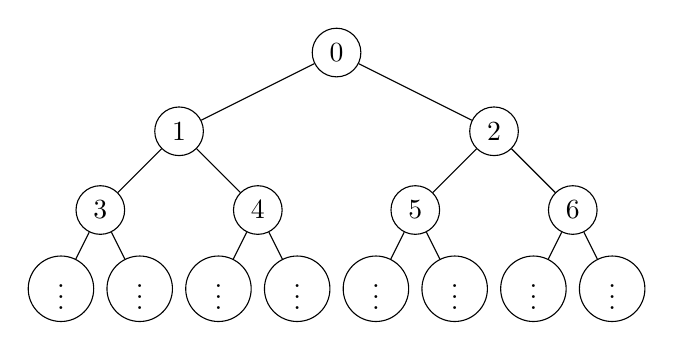
\begin{tikzpicture}[scale=0.5,level distance=2cm,
			level 1/.style={sibling distance=8cm},
			level 2/.style={sibling distance=4cm},
			level 3/.style={sibling distance=2cm},
			every node/.style={circle, draw, fill=white}]
		\node (0) {$0$}
		child {node (1) {$1$}
				child {node (3) {$3$}
						child {node {$\vdots$}}
						child {node {$\vdots$}}
					}
				child {node (4) {$4$}
						child {node {$\vdots$}}
						child {node {$\vdots$}}
					}
			}
		child {node (2) {$2$}
				child {node (5) {$5$}
						child {node {$\vdots$}}
						child {node {$\vdots$}}
					}
				child {node (6) {$6$}
						child {node {$\vdots$}}
						child {node {$\vdots$}}
					}
			};
	\end{tikzpicture}
\end{figure}

It is easy to see that the leaves will start with the value of $\left\lfloor\dfrac{2^{n + 1} - 1}{2}\right\rfloor$, where $n$ is the depth of the perfect binary tree.

\newpage
So to generate all the leaves of the perfect binary tree of depth $n$, we present the following algorithm:

\begin{algorithm}[hbt!]
	\caption{Perfect Binary Tree Leaves Generator}\label{alg:leaves-generator}
	\KwData{$n \geq 0$, where $n$ is the depth of the perfect binary tree}
	\KwResult{A perfect binary tree graph's leaves}

	\SetKwFunction{FMain}{perfect\_binary\_tree\_generator}

	\SetKwProg{Fn}{Function}{:}{}
	\Fn{\FMain{$n$}}{
		$num\_vertices \gets 2^{n + 1} - 1$\;
		$leaves \gets []$\;
		$last\_row\_start \gets floor(num\_vertices / 2)$\;
		\For{$vertex$ in range($last\_row\_start$, $num\_vertices$)}{
			$leaves$.append($vertex$)\;
		}
		\Return{$leaves$}
	}
\end{algorithm}

We then use the algorithm from ~\cite{Niskanen2003CliquerUG}Cliquer to generate a coclique of maximum cardinality for our perfect binary tree.

\begin{algorithm}[hbt!]
	\caption{Maximum Indpendent Set Algorithm}\label{alg:max-independent-set}
	\KwData{A perfect binary tree graph $T$}
	\KwResult{A maximum coclique of $T$}

	\SetKwFunction{FMain}{maximum\_coclique}

	\SetKwProg{Fn}{Function}{:}{}
	\Fn{\FMain{$T$}}{
		$cliquer \gets Cliquer(T)$\;
		\Return{$cliquer$.get\_maximum\_coclique()}
	}
\end{algorithm}

The next page shows the results of the algorithm for a perfect binary tree of depth 5. The X-axis denotes the vertice's labels (not the actual numbers) and the Y-axis denotes the cardinality of the stars centered around the vertices.

\begin{figure}[hbt!]
	\begin{subfigure}{.5\textwidth}
		\centering
		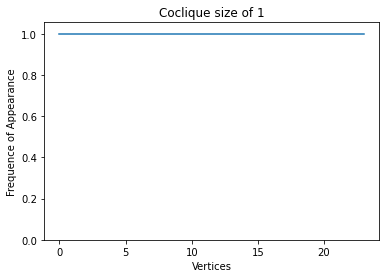
\includegraphics[width=1\linewidth]{size_1.png}
		\caption{coclique of size 1}
	\end{subfigure}
	\begin{subfigure}{.5\textwidth}
		\centering
		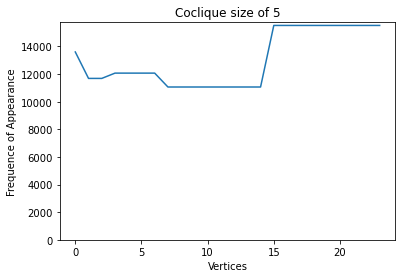
\includegraphics[width=1\linewidth]{size_5.png}
		\caption{coclique of size 5}
	\end{subfigure}
	\begin{subfigure}{.5\textwidth}
		\centering
		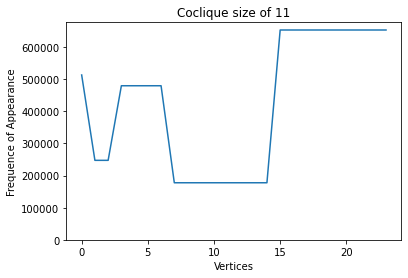
\includegraphics[width=1\linewidth]{size_11.png}
		\caption{coclique of size 11}
	\end{subfigure}
	\begin{subfigure}{.5\textwidth}
		\centering
		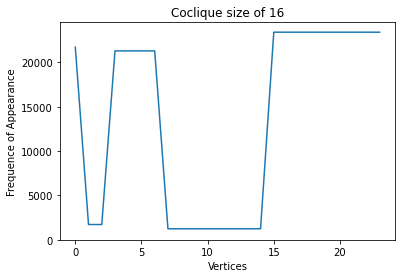
\includegraphics[width=1\linewidth]{size_16.png}
		\caption{coclique of size 16}
	\end{subfigure}
	\begin{subfigure}{.5\textwidth}
		\centering
		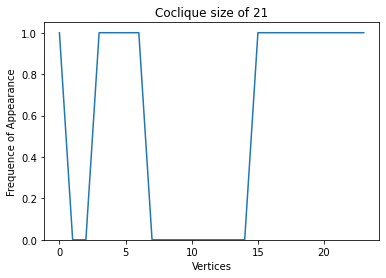
\includegraphics[width=1\linewidth]{size_21.png}
		\caption{coclique of size 21}
	\end{subfigure}
\end{figure}

The data shown in the figures above verifies that the Partial HK-Property holds for perfect binary trees of depth 5. The next step would be to verify this for perfect binary trees of depth 6 and 7.

However, the algorithm is very slow and inefficient and it scaled exponentially. Hence, running the algorithm for perfect binary trees of depth 6 and 7 would be very computationally expensive.

\newpage

\subsection{Inductive Conjectures}

From our observations from the algorithm, we note the following:

\begin{enumerate}
	\item The maximum coclique always seems to contain the last depth vertex set (All the leaves).
	\item The maximum coclique always seems to contain the root.
	\item The maximum coclique seems to start from the last depth vertex set and then move towards the root alternately.
\end{enumerate}

In essence, we observe that that maximum coclique number seems to follow this pattern:

If $T$ is our perfect binary tree of depth $d$, then
\begin{align*}
	\alpha(T) = 2^d + 2^{d-2} + \ldots
\end{align*}

When $d$ is even, we see that
\begin{align*}
	\alpha(T) = 2^d + 2^{d-2} + \ldots + 2^0
\end{align*}

When $d$ is odd, we see that
\begin{align*}
	\alpha(T) = 2^d + 2^{d-2} + \ldots + 2^1
\end{align*}

From our observations, we conjecture the following:

\begin{conjecture}
	For any perfect binary tree $T$ of depth $d$, the maximum coclique $\alpha(T)$ is given by
	\begin{align*}
		\alpha(T) = \sum_{i= 0}^{\left\lfloor\frac{d}{2}\right\rfloor} 2^{d - 2i}
	\end{align*}
\end{conjecture}

If this conjecture holds true, then we claim that:

\begin{claim}
	There is a unique maximum coclique set that contains all the leaves.
\end{claim}

Then, we can further conjecture that if we induct on $d$ and $k$ where $k \leq \alpha(T)$, we have:

\begin{conjecture}\label{conjecture_ptb_partial_hk}
	Let $T$ be a perfect binary tree of depth $d$. Let $r$ be the root of $T$. Then, for all possible values of $d$ and $k$, there exists a leaf $l$ of $T$ such that $|\mathcal{I}^k_T(v)| \leq |\mathcal{I}^k_T(l)|$ for each $v \in V\setminus{r}$.
\end{conjecture}

Note that \ref{conjecture_ptb_partial_hk} is basically the statement of the Partial HK-Property specifically for perfect binary trees.

\section{Conclusions}

To conclude, we believe that the Partial HK-Property holds for perfect binary trees. We have shown that the maximum coclique of a perfect binary tree follows a certain pattern and we have shown that the maximum coclique always seems to contain the leaves and the root.

We do have an idea of the proof and a proof sketch, however proving it will take some time and we plan to work on it in the future.

In addition, noting that a perfect binary tree is a special case of a perfect $k$-ary tree, we can conjecture that the Partial HK-Property holds for perfect $k$-ary trees as well, if our inductive conjecture holds true and is generalizable.

We also aim to explore other classes of $k$-ary trees and see if the Partial HK-Property holds for them as well in the future.

%%% Bibliography
\include{Bibliography}
\bibliographystyle{plain}
\addcontentsline{toc}{chapter}{Bibliography}
\bibliography{Bibliography}

\end{document}
